\chapter{Data and Methodology}
\label{chap:data_methodology}

This section details the data sources and methodological approaches employed in this thesis. It begins by describing the primary data source, the ICIJ Offshore Leaks Database, outlining its structure, content, strengths, and limitations. Subsequently, it discusses the external datasets used to provide contextual information. Finally, it introduces a novel methodology utilizing agentic AI to enrich the classification of intermediaries within the icij dataset.

\section{The ICIJ Offshore Leaks Database}
\label{sec:3_1}

The empirical core of this thesis rests upon the International Consortium of Investigative Journalists (ICIJ) Offshore Leaks Database. This resource serves as the primary data source, acting as a valuable, albeit imperfect, "proxy" for the opaque universe of offshore finance (cf. EU, 2017). The general idea underpinning its use here is that while any direct numerical estimates derived solely from the leaks (e.g., total wealth hidden) will surely be biased due to the data's inherent incompleteness, the qualitative nature of the interactions captured within the data – the patterns of relationships between clients, intermediaries, and jurisdictions – appears more reliable for understanding the structure and dynamics of the offshore system.

The use of the ICIJ Offshore Leaks Database for this type of research is increasingly established. For example, Alstadsæter et al. (2019), Londoño-Vélez \& Ávila-Mahecha (2021), and Chang et al. (2023a; 2023b). 

\section{External Data Sources}

\label{sec:3_2}

To contextualize the patterns observed within the ICIJ data, several external data sources are employed.

A key resource is the Historical Tax Havens Database (HTHD) developed by Laffitte (2024). This dataset documents the historical evolution of "offshore legal architecture," tracking the adoption of specific legal technologies (e.g., banking secrecy, IBCs) across tax havens over time. This dataset will be utilized to explore whether specific patterns observed in the ICIJ data – such as the prevalence of certain offshore instruments or shifts in intermediary activity – align temporally with the historical innovations documented in the HTHD.

The World Justice Project (WJP) Rule of Law Index provides comprehensive country-level metrics on governance. Its specific use is to investigate potential correlations between the home country's rule of law environment and the patterns of specialization or network positioning observed among the intermediaries serving clients from that country.

VDEM (Varieties of Democracy) Regime Type Data will be used exactly analogously.

Data from the World Inequality Database (WID), specifically metrics on wealth inequality at the country level, will also be incorporated.  This serves primarily to see if we can confirm some of the comparative statics Alstadsæter and Zucman derive, trying to verify whether there's anything to their supply-side model.

\section{Using Agentic AI to Scrape Data on Intermediaries.}
\label{sec:3_3}

A significant challenge in utilizing the ICIJ data for the purposes of this thesis is that intermediaries are often classified generically within the database. To analyze the specific roles and potential influence of different types of intermediaries, as outlined in the typology adapted from the EU (2017) paper (see Section 2.1.4), a more granular classification is required. To achieve this classification at scale, an approach employing agentic AI is utilized.

The core idea is to use an AI agent loop to automate the process of gathering information about and classifying the intermediaries listed in the ICIJ data. The basic workflow is illustrated in Figure \ref{fig:agent_loop_placeholder}.

\begin{figure}[htbp]
    \centering
    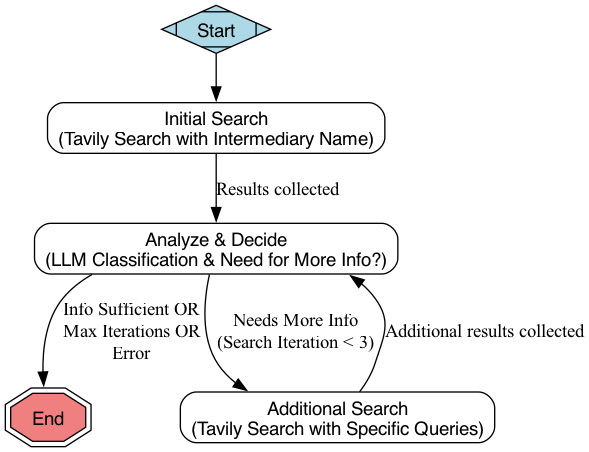
\includegraphics[width=0.8\textwidth]{agent_graph.png} 
    \caption{Agent Setup for Intermediary Classification}
    \label{fig:agent_loop_placeholder}
\end{figure}

In brief, the process involves an AI agent orchestrating online searches for each intermediary identified in the ICIJ data. It begins with generic searches, reads and interprets the initial results, and then formulates more specific search queries based on the information discovered or identified as lacking. This iterative process involves up to three search queries per intermediary, scouring the top 15 most relevant web results identified through query-result embedding similarity using the Tavily Search API (though the tool is relatively generic and it specifically is not very important). This effectively replaces the time-consuming need for manual searching of the intermediaries.

Based on the information gathered, the AI agent then classifies the intermediary according to the EU (2017) typology (Tax Expert, Legal Expert, Administrator, Investment Advisor), adding a few additional relevant fields (e.g., specific job title). Crucially, the agent also provides a confidence score for its classification judgment, allowing for filtering or weighting in subsequent analyses.

There are a few obvious limitations associated with this approach that warrant discussion:

Temporal Misalignment: A primary concern is that all online searches are conducted based on information available today, whereas the ICIJ data pertains to activities that may have occurred years or even decades prior. This introduces two potential issues:
    1.  The process might be biased towards identifying intermediaries who are still active or have a significant online presence currently.
    2.  It implicitly assumes that the role an intermediary plays today (as reflected online) is equivalent to the role they played at the time relevant to the ICIJ data.

Addressing the Limitations: While these issues are real, they are not prohibitive for their use in this thesis.
1. Regarding the first point (bias towards current intermediaries), this primarily impacts the coverage or statistical power of the classification – we may only be able to confidently classify a subset (e.g., 50\%) of all intermediaries. This is acceptable, provided the unclassifiable intermediaries are not systematically different in ways that correlate with the research questions. The issue becomes problematic only if there is a systematic bias in identifiability across types (e.g., if it is inherently much harder to find information online about legal experts compared to tax experts due to differing needs for discretion or public visibility).
2. Regarding the second point (role stability), the assumption that roles remain consistent is arguably less problematic. Given the highly specialized nature of functions like tax advisory, legal structuring, administration, and investment management within the offshore context, and the considerable barriers to entry (qualifications, reputation, networks) for each, frequent switching between these core roles by individuals or firms seems relatively unlikely.

In my view, it is the only pragmatically feasible method to do this given the constraints of this thesis.

(Note: LLMs have also been used to polish the text of this thesis.)
